\documentclass{article}
\newcommand\hmmax{0}
\newcommand\bmmax{0}
\usepackage{booktabs}

%% Language and font encodings
\usepackage[english]{babel}
\usepackage[utf8x]{inputenc}
\usepackage[T1]{fontenc}
\usepackage{gensymb}
\usepackage{pdfpages}

\usepackage[bitstream-charter]{mathdesign}
\let\circledS\undefined
%% Sets page size and margins
\usepackage[a4paper,top=2cm,bottom=2cm,left=1cm,right=1cm, marginparsep=1cm]{geometry}

%% Useful packages
\usepackage{amsmath}
\usepackage{bm}
\usepackage[makeroom]{cancel}
\usepackage{enumitem}
\usepackage{listings}
\usepackage{multirow}
\usepackage{amssymb}
\usepackage{float}
\usepackage{graphicx}
\usepackage{wrapfig}

\newcommand{\myq}[1]{%
	\vspace{1em}
	\noindent\underline{\emph{Exercise #1}}\vspace{0.25em}\linebreak
}

\DeclareMathAlphabet{\altmathcal}{OMS}{cmsy}{m}{n}

\usepackage[noend]{algpseudocode}
\usepackage{algorithm,algorithmicx}

\newcommand*\Let[2]{\State #1 $\gets$ #2}
\algrenewcommand\algorithmicrequire{}
\algrenewcommand\algorithmicensure{\textbf{Postcondition:}}

\title{\textbf{Reinforcement Learning: An Introduction}\\
\textit{Solutions: Chapter 5}
}
\author{Mrinank Sharma}

\begin{document}
\maketitle

\myq{5.1: Blackjack}
The estimated value is much higher if the player holds $20$ or $21$ as it is likely that the player wins since the dealer always plays to $17$ or higher (or bust), and the winner is whoever holds the higher sum. It is unlikely that the dealer can beat this count. 

The estimated value drops off when the dealer is holding an ace because an ace is an advantage because it acts as both $1$ and $11$, effectively giving the dealer an extra draw. 

The frontmost values are higher when the player has a usable ace with sum $12$, they are more likely to win. The player effectively gets more draws since if they draw a bad card, they can downgrade the ace to a $1$, and this is beneficial for avoiding getting bust which is likely with the current strategy. 

\myq{5.2: First-Visit vs. Every-Visit MC}
The results would be the same. It is not possible to a state to be revisited without a usable ace - the player sum can only go up and not say the same.

\textbf{Also, importantly, this game is properly Markov since the cards are drawn with replacement.}

\myq{5.3: Backup Diagram}
The backup diagram is the same as the backup diagram for estimating values except that now there is a value for each state-action pair. 

\myq{5.4: MCES}
Instead use arrays $\texttt{counts}[s, a] \leftarrow 0, \quad \forall s, a$ and $Q[s, a] \leftarrow 0, \quad \forall s, a$. Update $q$ using the incremental formula instead of averaging each time, also updating the counts as we go along. 

\myq{5.5: First-Visit vs. Every-Visit MC II}
The first visit value is $10$ whilst the every-visit value is $10/10 = 1$. Note that the actual value would be $V = 1/(1-p)$. 

\myq{5.6: Action-Value IS}
We now also condition on the first action being taken, therefore, the importance weights used start one step later (you could also follow the full derviation of IS to see this). The weighted important sampling estimate becomes:

\begin{align}
Q(s, a) = \frac{\sum_{t \in \altmathcal{T}(s, a)} \rho_{t+1:T(t)-1} G_t}{\sum_{t \in \altmathcal{T}(s, a)} \rho_{t+1:T(t)-1}},
\end{align}
i.e., visits are now to state-action pairs. 

\myq{5.7: Weighted Importance Sampling}
The weighted importance sampling estimate only includes episodes with behaviour from $b$ which is consisent with $\pi$. Our initial estimate of $0$ is close to the true value, so we start off performing pretty well. We start to perform worse as more of the runs end up some consisent behaviour, but since the weighted average has very few terms, the variance is high. As we generate more and more consistent episodes, the performing starts to increase again. 

Note that the policy is random, so its pretty unlikely to get consisent behaviour. Averaging over $100$ runs makes this graph much smoother. 

\myq{5.8: First-Visit vs. Every-Visit MC III}
I think that the variance would still be infinite. Let's imagine every-visit MC using standard importance sampling. Going to every-visit effectly adds additional terms to the estimate corresponding to places which weren't first visits. 

I'm not fully sure though. Since we are using every-visit, we are no longer summing independent random variables, so we cannot argue that the variance is the sum of individual variances. 

Even though we are no longer summing independent random variables (with an episode), there will not be a perfect negative correlation, so the variance (without rescaling) will increse. Therefore, it will remain infinite. We can imagine the worked example summation. Going to every-visit MC will add scaling and more positive terms. 

Maybe a nicer way of seeing this. The difference between first-visit and every-visit is the set $\altmathcal{T}(s)$. The variance sum now has additional terms in (and a new scaling factor). We already know the
 original terms sum to infinity. Now, they just sum to a larger amount. 
 
 \myq{5.9: MC policy evaluation: updated}
 This is a straightforward modification. Modify the \texttt{returns} array to store the current estimate and add an additional \texttt{counts} array. Replace the update formula with the standard incremental mean update.
 
 \myq{5.10: Weight-Average Update Rule}
 The update rule for $C_n$ gives, $C_n = \sum_{k=1}^n C_k$. 
 
 \begin{align}
 V_n &= \frac{\sum_{k=1}^{n-1} W_k G_k}{C_{n-1}} \\
 V_{n+1} &= \frac{\sum_{k=1}^{n-1} W_k G_k + W_n G_n }{C_n} \nonumber \\
 &= V_n + \frac{1}{C_n} [W_n G_n -  \underbrace{\sum_{k=1}^{n-1} W_k G_k}_{C_{n-1} V_n} - C_n V_n] \nonumber \\
 &= V_n + \frac{1}{C_n} [W_n G_n - {C_{n-1} V_n} - C_n V_n] \nonumber \\
 &= V_n + \frac{1}{C_n} [W_nG_n - {(C_{n} - W_{n}) V_n} - C_n V_n] \nonumber \\
 &= V_n + \frac{W_n}{C_n}[G_n - V_n]
 \end{align} 
 
 \myq{5.11: Off-policy MC Control}
 The probability is $1$ for the optimal action (according to the current $Q$). We basically directly substitute this in. 
 
 \myq{5.12: Racetrack Programming}
 This was quite a painful exercise. I ended up making a number of changes:
 \begin{itemize}[noitemsep]
 	\item Pessimistically initialise $Q$. Otherwise, the greedy policy is always a new action. This partially takes into account that it is difficult in general to reach the end. 
 	
 	\item I had issues with episodes taking a very long time to finish. This is not surprising - completely random actions are unlikely to reach the end. Combined with the issue of only learning from the tails of episodes, this made learning incredibly slow. I capped the episode length to $50$ and gave a large negative reward for reaching this length. 
 	
 	\item Learning slowly - I added penalities to hitting the wall in attempt to get things to learn faster. This penalty was the same penalty as the termination penalty (if the penalty is too small, the car will hit the wall in order to try and reach and initialisation state it knows how to finish from, avoiding the termination penalty and getting a better reward). 
 	
 	\item I didn't terminate episodes if the wall was hit, though I tried it. The problem with this approach, as I had it implemented, was that if you are going to hit the wall because you are bad a driving, you may as well hit it early and terminate the episode. 
 	
 	\item I added a variation on \emph{exploring starts}. Every few episodes, I evaluated the perform of the greedy policy from each starting position. I then picked the starting position of episodes with probaility proportial to how badly we did from that position. Learning tends to be slow anyway, and this helps to speed it up. 
 	
 	\item Balancing exploration is hard. If $\epsilon$ is too large, random actions are unlikely to lead to our policy changing much. If too small, we never explore. I ended up behaving purely randomly until the performance improved enough/ we found a policy which actually reached the finish line. After that point, I switched to $\epsilon=0.1$ in an attempt to improve this policy more.
 	
 	\item In this algorithm, the weights grow larger the longer the episodes are (significantly). Therefore, with noise, I think that good actions which were unfortunately were ignored end up performing very poorly and getting overweighted in the importance sampling algorithm. Because of this, I ended up turning off noise. I didn't properly check this hypothesis though. It might have been nice to inspect the IS weights and the episodes they corresponded to. 
 \end{itemize}

In general, I'm a bit uncomfortable with the fact that we don't update the importance weights retroactively even though our target policy (the current greedy policy) is constantly changing. I think this non-stationarity doesn't really help us learn much either. 

I suppose that I learnt the lesson that MC methods are very very slow! Especially off-policy seems to behave badly. 

Regardless, the greedy policies and trajectories can be found in Figures~\ref{fig:track_one} and  \ref{fig:track_two}. Most of these policies are pretty reasonable, but its also clear that by inspecting them, they are not optimal (e.g. could cut closer to corners e.t.c.). I ended up doing perhaps $10^5$ episodes or so, maybe a bit fewer. My exploring starts variant made this convergence significantly faster, especially for the second track. 

\begin{figure}
	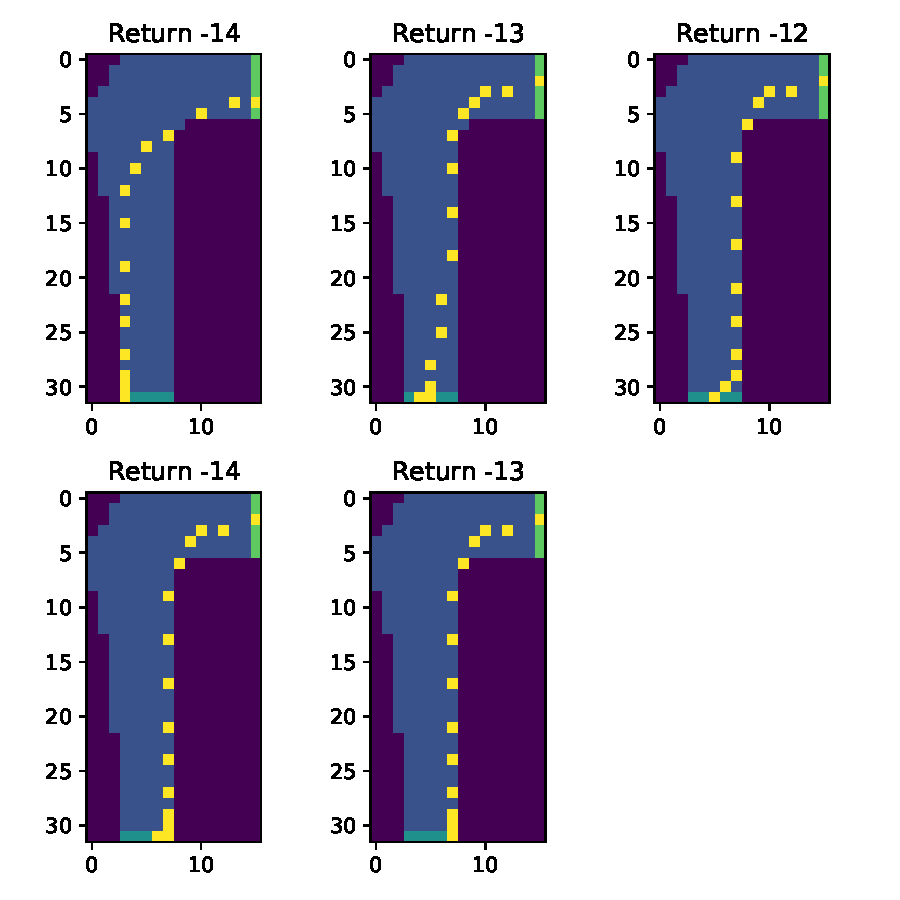
\includegraphics[width=\textwidth]{one}
	\centering
	\caption{\label{fig:track_one} First Track Sample Returns}
\end{figure}

\begin{figure}
	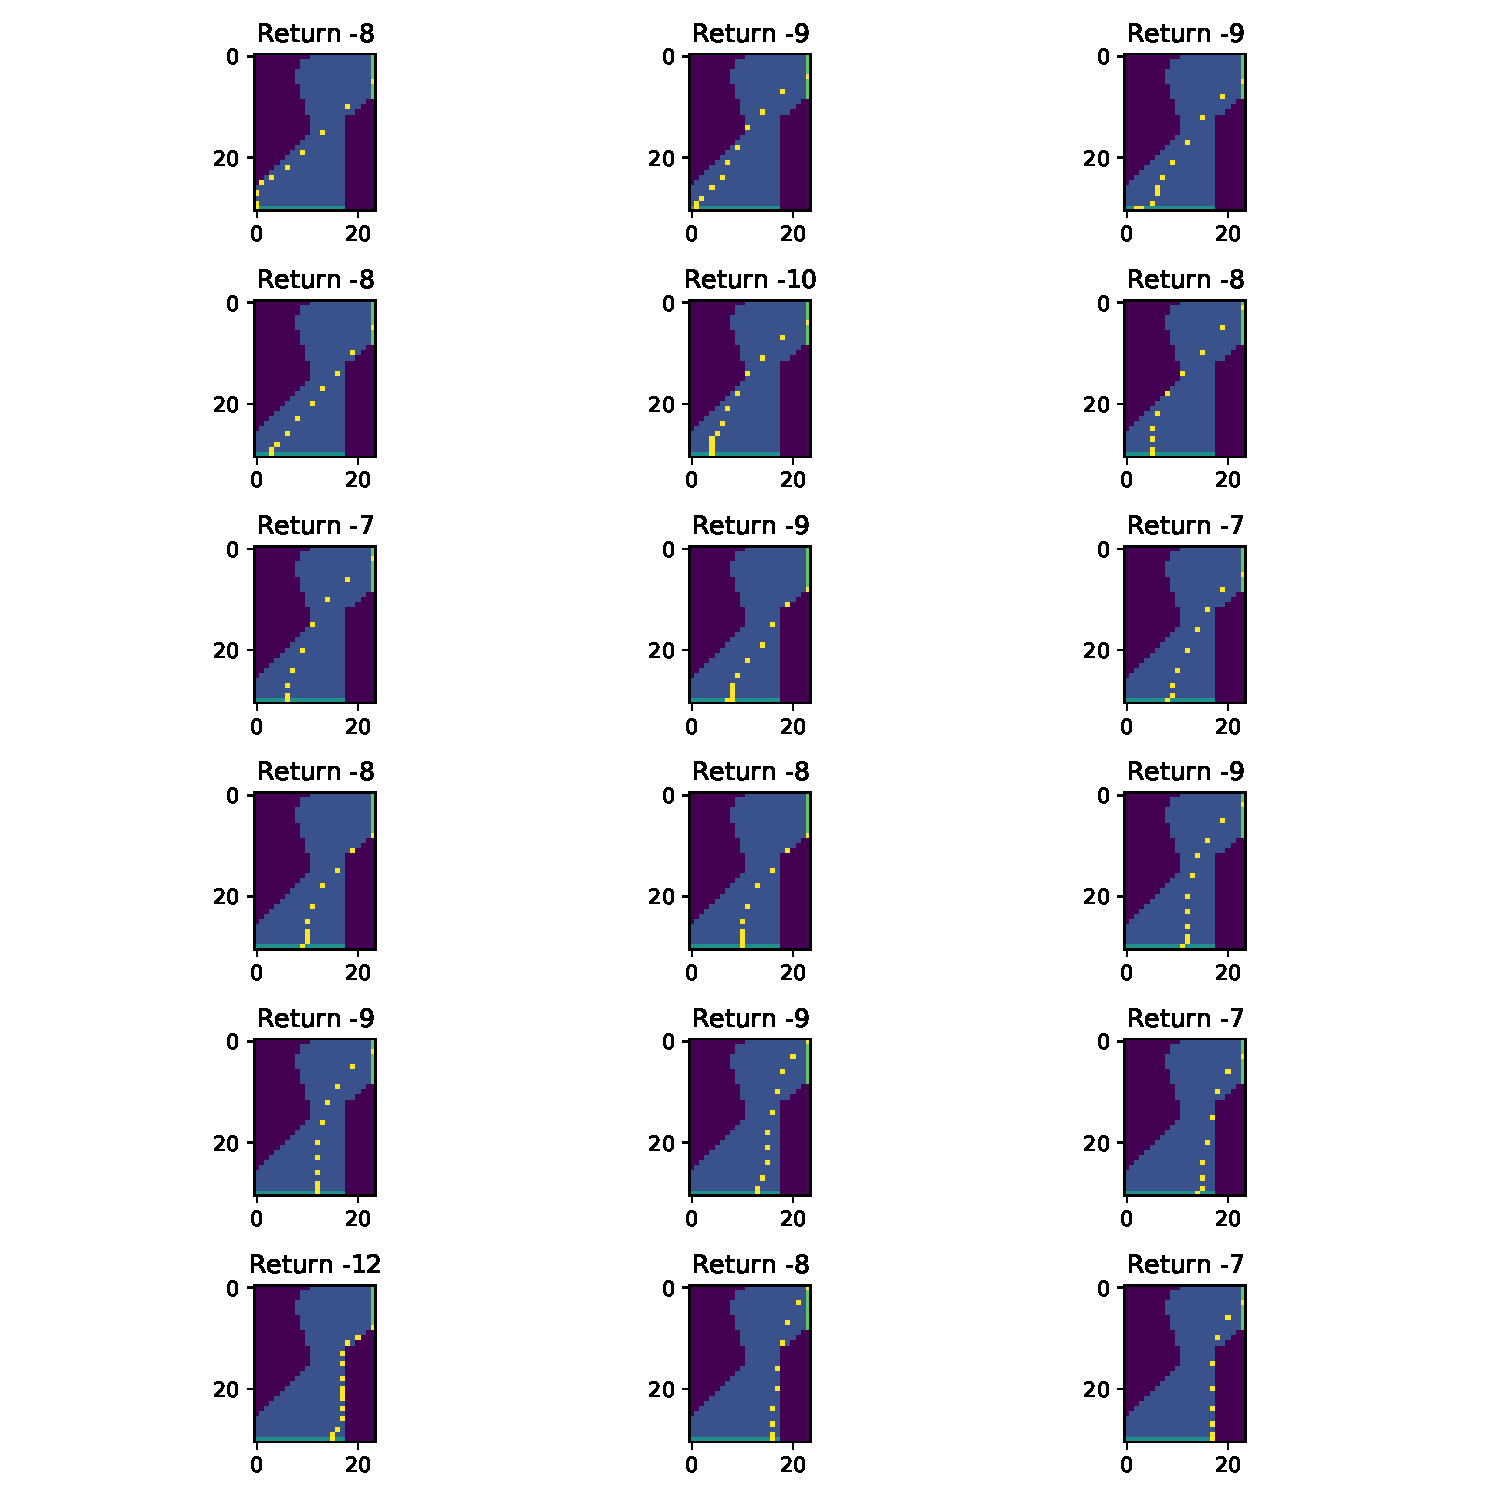
\includegraphics[width=\textwidth]{two}
	\centering
	\caption{\label{fig:track_two} Second Track Sample Returns}
\end{figure}

\myq{5.13: Per-Decision IS}
\begin{align}
\rho_{t:{T-1}} R_{t+1} = \prod_{i=t}^{T-1} \frac{\pi(A_i | S_i)}{b(A_i | S_i)} R_{t+1}
\end{align}
We want to show that we can neglect alot of the terms that come up in usual importance sampling. I'll show this for a value estimate, i.e., I'll condition on the state $S_t$. 
\begin{align}
\mathbb{E}_{b}[\rho_{t:{T-1}} R_{t+1} | S_t] &= \mathbb{E}_b\Big[ R_{t+1} \prod_{i=t}^{T-1} \frac{\pi(A_i | S_i)}{b(A_i | S_t)} | S_t \Big] \nonumber \\
&= \int \Big[ R_{t+1} \prod_{i=t}^{T-1} \frac{\pi(A_i | S_i)}{b(A_i | S_t)} \Big] p(S_{t+1}, R_{t+1} | S_t, A_t)b(A_t | S_t )b(A_{T-1} | S_{T-1} ) \prod_{i=t+1}^{T-2}p(S_{i+1}|S_i, A_i) b(A_i | S_i) d\lbrace A_i \rbrace_{i=t}^{T-1} d\lbrace S_i \rbrace_{i=t+1}^{T-1} \nonumber \\
&= \int R_{t+1} \prod_{i=t}^{T-1} \pi(A_i | S_i) p(S_{t+1}, R_{t+1} | S_t, A_t) \prod_{i=t+1}^{T-2}p(S_{i+1}|S_i, A_i) b(A_i | S_i)\ d\lbrace A_i \rbrace_{i=t}^{T-1} d\lbrace S_i \rbrace_{i=t+1}^{T-1} \nonumber \\
&= \int R_{t+1} \pi(A_t | S_t ) p(S_{t+1}, R_{t+1} | S_t, A_t) \Big[ \int \prod_{i=t+1}^{T-1} \pi(A_i | S_i) \prod_{i=t+1}^{T-2}p(S_{i+1}|S_i, A_i)\  d\lbrace A_i \rbrace_{i=t+1}^{T-1} d\lbrace S_i \rbrace_{i=t+2}^{T-1} \Big] dA_t dS_{t+1} \nonumber \\
&= \int R_{t+1} \pi(A_t | S_t ) p(S_{t+1}, R_{t+1} | S_t, A_t)  dA_t dS_{t+1} \nonumber \\
&= \int R_{t+1} \frac{\pi(A_t | S_t )}{b(A_t | S_t)} p(R_{t+1} | S_t, A_t)  b(A_t | S_t) dA_t  \nonumber \\
&= \mathbb{E}_{b}[\rho_{t:{t}} R_{t+1} | S_t]. 
\end{align}
This looks far more nasty than it actually is; effectively, write definition, expand out, marginalise to $1$ and then you are done. 

\myq{5.14: Discounting Aware IS}
This is more involved than it might first look. 

\begin{algorithm}[H]
	\caption{Off-policy Discount Aware MC Control
		\label{alg:off_policy_mc_control_discounted}}
	\begin{algorithmic}[1]
		\Require{
		\textbf{Input:} \Statex \hspace{\algorithmicindent} $\gamma \in [0, 1]$, discount rate. 	
	}
		
		\Statex
		\Require{
			\textbf{Initialisation:} \Statex \hspace{\algorithmicindent} $Q(s, a)$ arbitarily for all $s \in \altmathcal{S}, a \in \altmathcal{A}$. \Statex \hspace{\algorithmicindent} $C(s, a) \leftarrow 0 \text{ for all }s \in \altmathcal{S}, a \in \altmathcal{A}$ 
			\Statex \hspace{\algorithmicindent} $\pi(s) \leftarrow \arg \max_a Q(s, a)$, with ties broken \textbf{consistently}. 
		} 
		\Statex
		\Loop: 
		\Let{$b$}{any soft policy }		
		\State Generate an episode from under $b$: $\lbrace S_0, A_0, R_1, S_1, A_1, R_2, ..., S_{T-1}, A_{T-1}, R_T \rbrace$
		\For{$t \in \lbrace 1, 2, \dots, T-1 \rbrace$}:\Comment{Proceed forwards rather than backwards} 
		\Let{$\bar{G}$}{$0$}
		\Let{$W$}{$1$}
		\Let{$W_h$}{$1$}
		\Let{$C_h$}{0}
		\For{$h \in \lbrace{t+1, t+2, \ldots, T}\rbrace$}:
			\If{$A_{h-1} \neq \pi(S_{h-1})$}:
				\State \textbf{break}
			\Else:
			\Let{$W$}{$W \frac{1}{b(A_{h-1} | S_{h-1})}$} 
			\EndIf
			\Let{$\bar{G}$}{$\bar{G}+ R_h$} \Comment{Compute Forward Flat Reward}
			\If{$h=T$}:
			\Let{$W_h$}{$\gamma^{h-t-1}W$} 
			\Else:
				\Let{$W_h$}{$(1-\gamma) \gamma^{h-t-1}W$} 
			\EndIf
			\Let{$C(S_t, A_t)$}{$C(S_t, A_t) + W_h$} 
			\Let{$Q(S_t, A_t)$}{$Q(S_t, A_t) + \frac{W_h}{C(S_t, A_t)}[\bar{G} - Q(S_t, A_t)]$}  
		\EndFor
		\Let{$\pi(S_t)$}{$\arg \max_a Q(S_t, a)$ with ties broken consistently.}
		\EndFor
		\EndLoop
	\end{algorithmic}
\end{algorithm}
This algorithm looks very different from the other one. It calculates things forward rather than backwards, so ought to be able to learn well. 

If we put $\gamma=1$ in to this algorithm, it's almost the same, except that now we work forwards rather than backwards. I'm not fully sure, but it seems to work out to basically be the same. 

\end{document}